
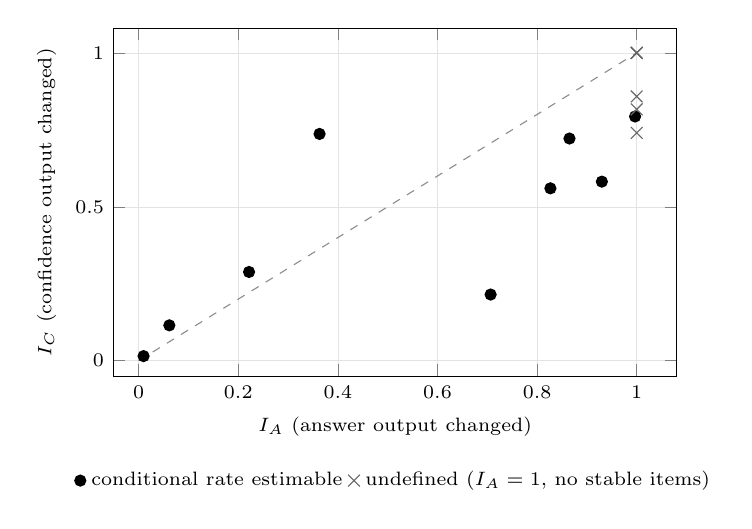
\begin{tikzpicture}
\begin{axis}[
  width=0.72\textwidth, height=6.0cm,
  xlabel={$I_A$ (answer output changed)},
  ylabel={$I_C$ (confidence output changed)},
  xmin=-0.05, xmax=1.08, ymin=-0.05, ymax=1.08,
  tick label style={font=\scriptsize}, label style={font=\scriptsize},
  legend style={font=\scriptsize, at={(0.5,-0.24)}, anchor=north, legend columns=2, draw=none},
  grid=major, grid style={gray!22,very thin}]
\addplot[domain=0:1, samples=2, black!45, dashed, forget plot] {x};
\addplot[only marks, mark=*, mark size=2.0pt, color=black] coordinates {(0.9967,0.7933) (0.9300,0.5817) (0.2217,0.2883) (0.0617,0.1150) (0.7067,0.2150) (0.3633,0.7367) (0.0100,0.0150) (0.8267,0.5600) (0.8650,0.7217)};
\addlegendentry{conditional rate estimable}
\addplot[only marks, mark=x, mark size=3.0pt, color=black!60] coordinates {(1.0000,1.0000) (1.0000,1.0000) (1.0000,1.0000) (1.0000,1.0000) (1.0000,0.8167) (1.0000,0.8583) (1.0000,0.7400)};
\addlegendentry{undefined ($I_A=1$, no stable items)}
\end{axis}
\end{tikzpicture}
